\chapter{Git} \label{ch:git}

Git is a distributed version control system for tracking changes during the software development, and it can be used on multiple platforms including Windows, Unix/Linux and MacOS. This chapter introduces the basic use of Git on a local Linux machine and with a remote repository host server such as GitHub. 

Git-based version control is widely used in association with \myabb{Continuous Integration and Continuous Deployment}{CI/CD}. CI/CD is an important concept in nowadays software development and deployment. GitHub Actions is GitHub's CI/CD solution and it is also briefly introduced.

\section{Introduction}

\mync{Git}, initially created by Linus Trovalds in 2005, is a distributed version control system for tracking changes in source code and files. It is helpful with maintaining data integrity during the collaborative development of software in distributed non-linear workflows. Git is free and open-source under GNU general public license.

Git introduces \mync{Git repository}, which refers to the ``ecosystem'' Git uses to manage a project. This refers to the \verb|.git| file associated with each Git-managed project, using which Git traces the development of the project. 

With Git, all computers participating in the software development store a copy of the full-fledged Git repository locally with complete history, and they can synchronize with centralized remote servers. It introduces \mync{branch} to manage the concurrent development of different features of the project, where the main branch (also known as master branch) is the stable and shared repository among everyone, and the child branches (also known as feature branches) are copies of the main branch where individual features can be developed. For a feature branch, once its developed feature is approved, it can be merged back to the main branch. A demonstration is given in Fig. \ref{ch:sma:fig:gitflow}.
\begin{figure}[htbp]
	\centering
	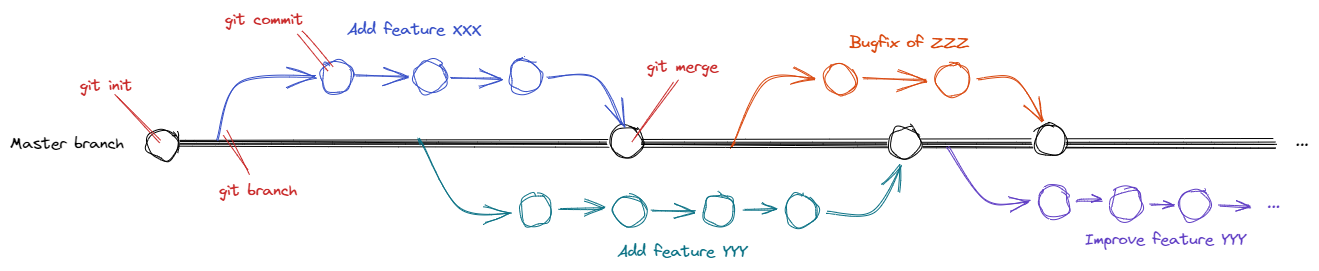
\includegraphics[width=350pt]{chapters/part-3/figures/gitflow.png}
	\caption{Git for software development management.} \label{ch:sma:fig:gitflow}
\end{figure}

CLI is often used to manage a Git repository. Some commonly used commands are shown in Fig. \ref{ch:sma:fig:gitflow} with more to be introduced later. Notice that a graphical user interface is also available. However, in the scope of this notebook, command line is mostly used.

\section{Git Setup}

Git and its relevant documents can be obtained from its official website \cite{git2025}. In many Linux distributions, Git is pre-installed. If Git is missing, follow the instructions on the official website to install it. The installation procedure may differ with different Linux distributions.

To install Git on RHEL, simply use
\begin{lstlisting}
$ sudo dnf install git-all
\end{lstlisting}

Upon successful installation, it is recommended to use \verb|git config| for the necessary basic configurations such as the username and user email. Without these configurations, Git cannot run normally.

Notice that there are two types of configurations, namely the global configurations which apply to the machine and the user, and the repository configurations which apply to a particular Git repository. By default, the global level configurations are stored under \verb|~/.gitconfig| and the repository configurations \verb|./.git/config| of the repository, respectively. It is recommended to use Git CLI to setup the configurations, rather than modifying the files directly.

To add user name and email to the global configuration, use
\begin{lstlisting}
$ git config --global user.name '<user name>'
$ git config --global user.email '<user email>'
\end{lstlisting}
To retrieve the global configuration, use
\begin{lstlisting}
$ git config --global -l
\end{lstlisting}
To revoke a global configuration, use
\begin{lstlisting}
$ git config --global --unset <configuration>
\end{lstlisting}
For example,
\begin{lstlisting}
$ git config --global --unset user.name
\end{lstlisting}
removes the user name.

More details about \verb|git config| can be found at \cite{git2025reference}.

\section{Local Repository Management}

Git CLI can manage both local and remote repositories, and can synchronize them bidirectionally. This section studies local repository management.

\subsection{Initialization of a Repository}

Navigate to the project directory. Use the following command to create a new Git repository for the project.
\begin{lstlisting}
$ git init
\end{lstlisting}
When the above command is applied, Git creates \verb|.git| directory in the working directory. From this point onward, Git monitors everything that happens inside this directory and its sub-directories and tries to track any change to the files, unless otherwise configured specifically. Many Git commands such as \verb|git status| become available. More details are introduced in the remaining of the section.

\subsection{Version Tracking}

For simplicity, assume that there is only one branch in the repository, namely the main branch. Notice that when there are multiple branches, the version-tracking works the same for each and every branch in a separate and independent manner. The mechanism behind version tracking is briefly introduced as follows.

The project directory is split into two parts, outside \verb|./.git/| the workspace, and inside \verb|./.git/| the Git repository. The workspace has the up-to-date project contents and it is directly managed by the user, while Git repository is managed by Git. The user should not manage the repository directly unless using the Git interface.

Inside the Git repository are metadata of the workspace files such as which files have been changed since the last deployment, etc. It also stores a full back up of every historical versions of the project (with powerful compressing mechanisms, of course). It is worth mentioning that instead of recording the changes of a file from version to version, Git records the snapshot of the file in every version, unless it is left untouched between two consecutive versions.

Figure \ref{ch:sma:fig:gitbasics} gives a demonstration of how Git manages the project directory. Git categorizes files in the workspace into the following states: untracked, modified (unstaged), staged, and unmodified. This is shown by Fig. \ref{ch:sma:fig:gitbasics}. A brief explanation of each state is given in Table \ref{ch:sma:tab:gitbasics}. More details are given later.

\begin{figure}[!htb]
	\centering
	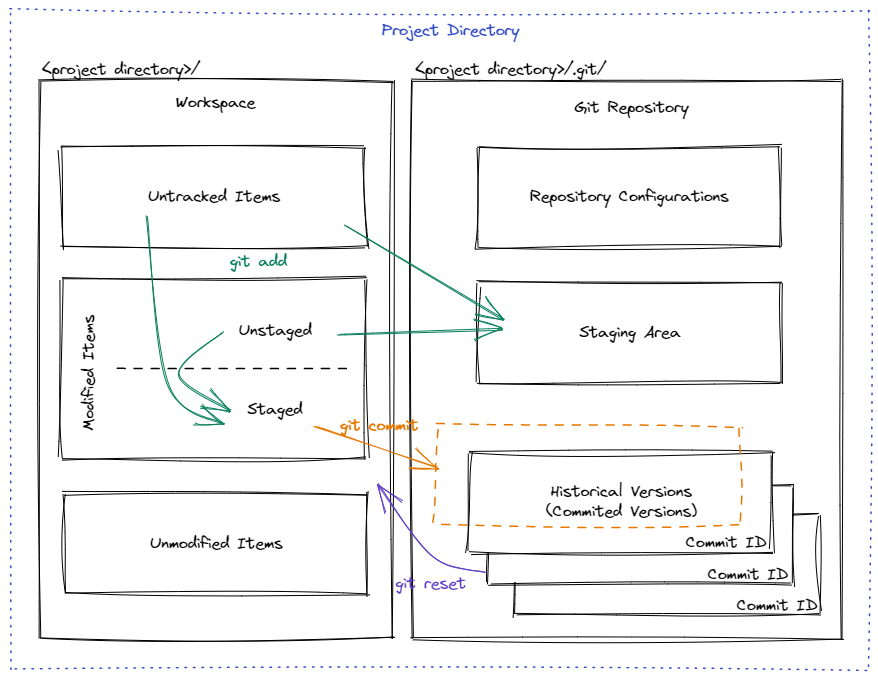
\includegraphics[width=350pt]{chapters/part-3/figures/gitbasics.png}
	\caption{The project directory managed by Git.} \label{ch:sma:fig:gitbasics}
\end{figure}

\begin{table}[!htb]
	\centering \caption{Different file status in a Git managed project.}\label{ch:sma:tab:gitbasics}
	\begin{tabularx}{\textwidth}{lX}
		\hline
		Status & Description \\ \hline
		Untracked & Newly added or renamed items in the project directory.  \\ 
		Modified (Unstaged) & Modified items from the last version that has not been registered in the staging area.  \\ 
		Modified (Staged) & Modified items from the last version that has been registered in the staging area. Notice that an untracked item can be staged directly, skipping ``modified (unstaged)'' step. Use \verb|git add| to stage items. \\ 
		Unmodified & Unmodified items from the last commit. \\ \hline
	\end{tabularx}
\end{table}

Use \verb|git status| to check the file states in the project. An example is given below.
\begin{lstlisting}
$ git status
On branch master

Changes to be committed:
  (use "git restore --staged <file>..." to unstage)
	modified:   chapters/ch-software-management-advanced/ch.tex

Changes not staged for commit:
  (use "git add <file>..." to update what will be committed)
  (use "git restore <file>..." to discard changes in working directory)
	modified:   appendix/ap.tex
	modified:   main.pdf

Untracked files:
  (use "git add <file>..." to include in what will be committed)
	chapters/ch-software-management-advanced/figures/
\end{lstlisting}
where \verb|ch.tex| is a modified (staged) item; \verb|ap.tex| and \verb|main.pdf| modified (unstaged) items, and \verb|figures/| an untracked item. Notice that unmodified files are not shown.

It takes a two-step procedure to back up the project in the Git repository. In the first step, the user flags the changed items (either newly added, renamed, or modified) to be backed up in the next version. In the second step, the user actually backs up the items. The first and second steps are called ``stage'' and ``commit'' respectively. Notice that it is possible to run a single line of command to execute both steps, but logically it still takes two steps.

Git tracks the name and content of the items that the user has staged in the ``staging area'' as shown in Fig. \ref{ch:sma:fig:gitbasics}. Think of staging items as taking a snapshot of the items. However, the snapshot at this stage is temporary and has not been backed up in the repository yet. The actual backup happens later when the staged items are committed. To stage an item, use
\begin{lstlisting}
$ git add <item name>
\end{lstlisting}
which registers the item in the staging area, thus also changes its status from untracked or modified (unstaged) to modified (staged). If an item is modified after it has been staged, Git will distinguish the ``staged portion'' and ``unstaged portion'' of that item. If using \verb|git status| to check its status, the item will be listed as both staged and unstaged. Unstaged items, either untracked or modified, will remain its status after the commit. Sometimes for convenience, \verb|git add -A| can be used to add all untracked or modified items to the staging area.

Use \verb|git commit| to commit the staged items and back them up in the repository as follows.
\begin{lstlisting}
$ git commit [<item name>]
\end{lstlisting}
The above command commits the project and creates a version in the Git repository. It is possible to specify items, in which case Git only commits the specified items and leave the rest items as they are. A commit ID is automatically assigned to the commit. Notice that the user will be asked to provide a ``comment message'' with the commit, which should be used to briefly explain what has been changed in this commit.

A flag \verb|-a| with \verb|git commit| stages all changes made to the project, then implements the commit command. A flag \verb|-m| simplifies the message recording process and allows the user to key in the message directly after the command. An example is given below.
\begin{lstlisting}
$ git status
On branch master

Changes not staged for commit:
  (use "git add <file>..." to update what will be committed)
  (use "git restore <file>..." to discard changes in working directory)
        modified:   A Notebook on Linux/chapters/ch-software-management-advanced/ch.tex
        modified:   A Notebook on Linux/main.pdf

no changes added to commit (use "git add" and/or "git commit -a")

$ git commit -am "add introduction to git command"
[master e2e977e] add introduction to git command
 2 files changed, 5 insertions(+), 4 deletions(-)

$ git status
On branch master

nothing to commit, working tree clean
\end{lstlisting}

To check the commit logs, i.e., all historical commits including their associated timestamps, authors, commit IDs and comment messages, use \verb|git log| as shown in the example below. Notice that the commit logs can be very long. Only a few commits are given for illustration purpose.
\begin{lstlisting}
$ git log
commit e3475e673d8c2a087de6b4423188c51e80af3e5d (HEAD -> master)
Author: sunlu <sunlu.electric@gmail.com>
Date:   Wed Aug 31 15:16:52 2022 +0800

    git

commit 3ab6d1473a7e48d4d890509ddb5a87274c023e6c
Author: sunlu <sunlu.electric@gmail.com>
Date:   Tue Aug 30 15:50:06 2022 +0800

    k8s

commit f6a1e3d779305e966602ecd7589c05f56dd2ad0f
Author: sunlu <sunlu.electric@gmail.com>
Date:   Mon Aug 29 16:31:18 2022 +0800

    more on docker and kubernetes

commit e2de5b28db7982f57d0ad51361d5161b884f2efe
Author: sunlu <sunlu.electric@gmail.com>
Date:   Sun Aug 28 21:38:48 2022 +0800

    add docker sections
\end{lstlisting}
where notice that \verb|HEAD| is a reference that points to the latest commit in a branch. Filters can be added as optional arguments for the \verb|git log| command. More details are given at \cite{git2025reference}.

And finally, to restore to a previous commit version, use \verb|git reset| or \verb|git revert|. Notice that \verb|git reset| and \verb|git revert| can both be used to restore the workspace to a previous stage, but they differ significantly. Their differences are introduced below.

Command \verb|git reset| erases the past commits in the local branch. This should not pose any problem if the erased commits have not spread everywhere else. Therefore, \verb|git reset| is helpful for local repositories without upstreams, or for modifications that have not been pushed to the upstreams. 

The command \verb|git reset| is often used as follows.
\begin{lstlisting}
$ git reset <option> <commit ID>
\end{lstlisting}
where \verb|<option>| is often \verb|--hard|, \verb|--mixed| or \verb|--soft|, and \verb|<commit ID>| can be the ID of any commit in the git log, or for shortcut \verb|HEAD| the current position of the HEAD (commit pointer), usually the latest commit.

The options \verb|--hard|, \verb|--mixed| and \verb|--soft| work differently. All these options move HEAD to the specified commit, and remove all commits afterwards from the repository. The \verb|--hard| option reverts the workspace back to when the specified commit happened (meaning that there would be no way to undo the reset command). Both \verb|--mixed| and \verb|--soft| do not change the workspace. The \verb|--mixed| option leaves all the changes from the specified commit to today as unstaged, while \verb|--soft| leaves them as staged. If no \verb|--hard|, \verb|--mixed| or \verb|--soft| is given, \verb|--mixed| will be used as the default option.

Notice that \verb|git reset| may pose an issue if the commits to be erased have already spread to the upstreams. This is because the erased commits in the local repository by \verb|git reset| will be reverted back the next time the local repository synchronizes with its upstream, where the commits in the upstream will be considered more up to the date, hence pulled to the local repository.

In such cases, consider using \verb|git revert| instead. Syntax wise they work similarly. Instead of erase the history, \verb|git revert| creates a new commit whose content is copied and pasted from a past commit.

\subsection{Branch Management}

\mync{Git branch} is a core concept and feature of Git, and it plays an important role in collaborative development of a project. 

There are two types of branches, namely the local branch and the remote branch. Remote branch is often associated with local branches, and play as the upstream mirror of the later for sharing and synchronizing the project development across machines. This section focuses on local branches. Remote branches will be introduced in Section \ref{ch:sma:sec:rrm}.

To list down all the local branches, use
\begin{lstlisting}
$ git branch
\end{lstlisting}
and the current working branch will be highlighted. The current working branch is also referred as the ``head branch'' or the ``active branch''.

To create a new branch from the current branch, and to delete a branch, use
\begin{lstlisting}
$ git branch <new branch name> [<commit ID>]
$ git branch -d <branch name>
\end{lstlisting}
respectively. The optional \verb|<commit ID>| when creating a new branch allows the user to create a branch on top of a specified historical commit instead of the latest commit.

To rename a branch, use
\begin{lstlisting}
$ git branch -m [<old branch name>] <new branch name>
\end{lstlisting}
where if no \verb|<old branch name>| is specified, the current working branch will be renamed.

To switch to a different working branch, use \verb|git checkout| or \verb|git switch| as follows.
\begin{lstlisting}
$ git checkout <branch name>
$ git switch <branch name>
\end{lstlisting}
Notice that when there are uncommitted changes in the current branch, Git may forbid the user to switch to another branch (the rules are too complicated to be explained here). Therefore, it is recommended to commit the changes before switching to a different branch. When switching to another branch, the workspace will change accordingly to the target branch.

To merge a branch back to the current branch, use
\begin{lstlisting}
$ git merge <branch name>
\end{lstlisting}
and fill in the comments accordingly. A use case of the command is to merge the features developed in a feature branch to the main branch, after a pull request is raised by the feature branch. To do that, checkout to the main branch, and use
\begin{lstlisting}
$ git merge <feature branch name>
\end{lstlisting}
By default, Git automatically deletes the merged branch. This behavior can be changed in the configuration. More about pull request are introduced in Section \ref{sec:pull_request}.

An alternative way of integrating two branches is \verb|git rebase|, which ``rewires'' the two branches into a linear single branch. Use \verb|git rebase| as follows.
\begin{lstlisting}
$ git rebase <branch name>
\end{lstlisting}
A demonstrative Fig. \ref{ch:sma:fig:gitrebase} explains the differences between \verb|git merge| and \verb|git rebase|. It is clear from Fig. \ref{ch:sma:fig:gitrebase} that by using \verb|git rebase|, all feature commits are integrated into the master repositories to form a single repository tracking line, which differs largely from \verb|git merge|.
\begin{figure}[!htb]
	\centering
	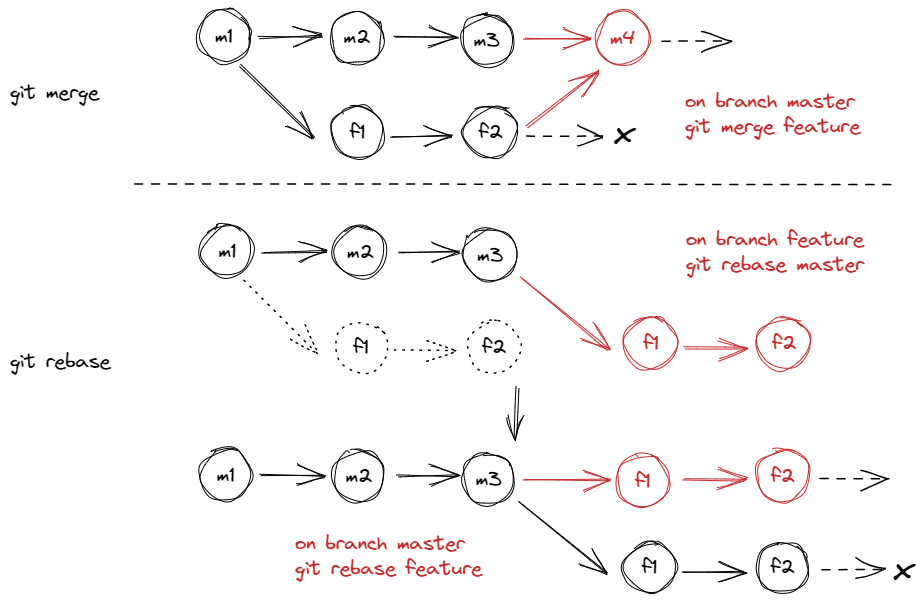
\includegraphics[width=350pt]{chapters/part-3/figures/gitrebase.png}
	\caption{Two approaches of integrating branches, \texttt{git merge} VS \texttt{git rebase}. In the \texttt{git rebase} example, two rebase commands are executed consecutively, the first on the feature branch and second the main branch.} \label{ch:sma:fig:gitrebase}
\end{figure}

An intuitive way to understand \verb|git rebase| is given as follows. Imagine two branches $A$ and $B$ that have diverged from the same commit $O$. On branch $A$, execute \verb|git rebase B|. Here is a step-by-step breakdown of what happens:
\begin{enumerate}
	\item Identify common ancestor of the current branch $A$ and the rebase branch $B$, which is commit $O$ in this example.
	\item Back up commits happened on branch $A$ since commit $O$. Assume they are commits $A_1$, $A_2$, ..., $A_n$.
	\item Reset branch $A$ to Branch $B$ and $A$ now starts from the tip of $B$.
	\item Reapply commits $A_1$, $A_2$, ..., $A_n$ on the reset $A$ in a sequential manner. In the case where there are conflicts when reapplying $A_1$, $A_2$, ..., $A_n$, the user needs to jump in and resolve them manually.
\end{enumerate}
After the rebase operation, the history of branch $A$ appears as if it was developed sequentially from the end of branch $B$, effectively integrating the changes of $B$ into $A$ in a linear history.

\section{Remote Repository Management} \label{ch:sma:sec:rrm}

Git hosting servers provide platforms for the developers to share their Git repositories and collaboratively develop projects. There are many cloud-based public Git hosting service providers such as GitHub, GitLab and Gitee. In this section, GitHub is studied. Notice that under the scope of this section, only basic functions are introduced and they should apply similarly to other Git hoisting service providers.   

An HTTPS URL is associated with each remote repository on GitHub, for example \textit{https://github.com/torvalds/linux.git} for Linux kernel. This URL can be used to download the remote repository to a local machine, or to link (synchronize) a local repository with that remote repository.

\subsection{Clone and Pull: from Remote to Local}

Consider the case where there is already a remote repository, either under the user's GitHub account or from the community. The user can clone the repository, i.e., make a local copy of the repository, as follows.

Use
\begin{lstlisting}
$ git clone <repository URL> [<local directory>]
\end{lstlisting}
where \verb|repository URL| can be the HTTPS URL of the repository. 

Git is able to trace the URL from which a local repository is cloned. To maintain the local repository up-to-date with the remote repository, regularly use
\begin{lstlisting}
$ git remote update
$ git pull
\end{lstlisting}
to pull the latest update.

\begin{shortbox}
\Boxhead{Should I use \texttt{git pull} or \texttt{git fetch}?}

One may argue whether it is a good idea to use \verb|git pull|. Although convenient, \verb|git pull| is an integration of two commands, \verb|git fetch| and \verb|git merge| (or \verb|git rebase|) executed sequentially. It may be ``safer'' to manually run the two commands separately.

With that being said, if the user simply wants to keep a well-maintained community project up to date, \verb|git pull| should work just alright.
\end{shortbox}

However, this does not guarantee that the user can perform a \verb|git push| command to push changes made in the local repository back to the remote source. For that, additional authentication is often required. More about \verb|git push| and remote repository authentication methods are introduced in later sections.

\subsection{Push: from Local to Remote}

Consider a scenario where you have a well-developed local Git repository, and you have just created an empty remote repository on GitHub. The goal is to link the remote repository with the local repository so that changes can be synchronized.

To establish a connection between the local and remote repositories, navigate to the local repository and run
\begin{lstlisting}
$ git remote add <remote-name> <remote-repository-URL>
\end{lstlisting}
This command registers the remote repository's URL in the local Git configuration. A commonly used remote name is ``origin''.

Note that if the local repository was originally created by cloning an existing remote repository, then ``origin'' is likely already set to the source of the clone. Use \verb|git remote -v| to check the registered remote source.

The next step is to associate the current working branch with a branch in the remote repository. This ensures that git pull and git push operate on the correct branch by default. This can be done as follows.
\begin{lstlisting}
$ git branch --set-upstream-to=<remote-name>/<branch-name>
\end{lstlisting}
Alternatively, the upstream branch can be set when pushing it for the first time using
\begin{lstlisting}
$ git push --set-upstream <remote-name> <branch-name>
\end{lstlisting}

Once the upstream is configured, the user can use 
\begin{lstlisting}
$ git push
\end{lstlisting}
to push the changes in the local remository to the remote upstream. If there is no remote branch with the same branch name as the local repository, a remote branch with that name will be created when the local branch is pushed.

\begin{shortbox}
\Boxhead{The Names of Corresponding Local and Remote Branches}

A local branch and its corresponding remote branch usually have the same name by default, but this is not necessarily always the case. To set an upstream with a different name, use
\begin{lstlisting}
$ git branch --set-upstream-to=\
<remote-name>/<remote-branch-name> <local-branch-name>
\end{lstlisting}
or
\begin{lstlisting}
$ git push <remote-name> <local-branch-name>:<remote-branch-name>
\end{lstlisting}

\end{shortbox}

When performing \texttt{git push} for the first time, authentication is required. This allows GitHub or another hosting service to verify the identity of the user before accepting changes. Common authentication methods include
\begin{itemize}
    \item Username and password authentication. Notice that this has been deprecated by GitHub in favor of token authentication.
    \item Personal access tokens.
    \item SSH key authentication.
\end{itemize}

\section{Pull Request} \label{sec:pull_request}

In a collaborative project, the main branch is managed very carefully because everything on that branch will affect the project in the production environment. There is often a group of senior developers maintaining the main branch. Any code to be added to the main branch must be reviewed by one or a few of them.

When a feature branch wants the features developed on that branch to be merged to the main branch, it does not push the changes to the main branch directly. Instead, the owner of the feature branch needs to raise a ``pull request'' from the GitHub dashboard. As its name suggests, it requests the main branch to pull the updates from the feature branch. The main branch maintenance team will then view and check the feature branch, making sure that everything is correct before they approve the merging.

If the pull request is approved, GitHub will perform the merge in the cloud. Neither the owner of the feature branch nor the maintenance team needs to run the merge manually.

\section{Collaborative Development in Practice}

This section introduces the common procedures an individual contributor follows to make improvements to a community project. We assume that an individual contributor has found a community project hosted on GitHub that interests him and believes he can update the code to improve it.

The following is a general flow where an individual contributor helps with improving an open-source project.
\begin{enumerate}
	\item The contributor forks the project to his own GitHub account.
	\item The contributor clones a copy of the project from his own GitHub account to his own machine.
	\item The contributor creates a new branch about the feature he wants to add or improve.
	\item The contributor develops the feature on the branch.
	\item The contributor commits the development and pushes the commit to the forked repository.
	\item The contributor submits a pull request to the maintenance team of the community project.
	\item The maintenance team receives the pull request and reviews the changes made to the code in the developer's forked repository.
	\item The maintenance team either sends feedback to the contributor for further clarification, or pulls the changes from the developer's forked repository and merge the new feature branch with the existing branches.
\end{enumerate}

As a first step, the contributor forks the project into his own GitHub account. This creates a copy of the community project under the contributor’s account, giving him full control over the forked repository. He is free to make or test any modifications without affecting the original project.

Although a fork is treated as a separate repository in many ways, GitHub tracks the relationship between the fork and the original project. This allows the contributor to later request that his modifications be merged back into the original community repository. Using the fork approach also acknowledges the contributions of the original authors, making it a more respectful and transparent process compared to simply downloading the project and uploading it as a new repository under the contributor's account.

After forking, the contributor can clone the project from his GitHub account to the local computer. He can then modify and test the code locally. Once the changes are made, he can upload the updated code to their forked repository using
\begin{lstlisting}
$ git push
\end{lstlisting}

\begin{mdframed}
\textbf{Is it possible to push to the original repository directly?}

It is worth mentioning that if \verb|git fork| were not used to fork the repository to the contributor's GitHub account, this \verb|git push| will run into a permission issue. This is because the contributor does not possess ownership to the original repository, hence prevented from modifying it.

It is not recommended, but possible, that the contributor can contact the owner of the repository and ask for permission. The owner of the original repository can invite the contributor as a collaborator of the project. In that case, the contributor will be able to create and push branches to the original repository. Notice that likely the contributor cannot merge his branch to the main branch and still needs pull request to do so.

\end{mdframed}

When the forked repository has been updated with improvements, the contributor can create a pull request in the original community repository. The maintainers of the community project will review the pull request, evaluate the modifications, and either reject it, provide feedback, or approve it for merging.

It is possible that while the contributor is working on their changes, new features or updates are introduced in the original community project. To keep their fork up-to-date, the contributor can add the original repository as a second remote, commonly named ``upstream''. The forked repository under their account is typically referred to as ``origin''. To synchronize with the original repository, the contributor can execute the following commands.
\begin{lstlisting}
$ git fetch upstream
$ git checkout master
$ git rebase upstream/master
\end{lstlisting}

By following this procedure, the contributor ensures that his work remains aligned with the latest developments in the community project, reducing the chances of conflicts and making their contributions easier to integrate.

\section{GitHub Actions}

GitHub has been an amazing platform for managing software projects, especially open-source collaborative projects. In the early days when CI/CD was not enabled in GitHub, developers used third-party CI/CD tools such as Jenkins and Travis CI in conjunction with GitHub for fast and convenient integration and deployment. Lately, GitHub introduced \mync{GitHub Actions}, its own CI/CD solution, as a response to developers' requests.

GitHub Actions is essentially a workflow automation service that allows the user to define a sequence of actions that can be triggered by timers or repository-related events. The workflow can be used for both CI/CD tasks such as code building, testing and deployment, and for managing the repository such as adding labels. Machine-readable instruction files are used to configure the workflow and they are included in the repository and managed together with the source code.

This section gives a brief introduction to GitHub Actions. More details are given in \cite{git2025reference}.

\subsection{Workflow Building Blocks}

The basic building blocks of GitHub Actions include
\begin{itemize}
	\item Workflows
	\item Jobs
	\item Steps
\end{itemize}
A demonstrative plot is given in Fig. \ref{fig:actions_workflow}.
\begin{figure}[!htb]
	\centering
	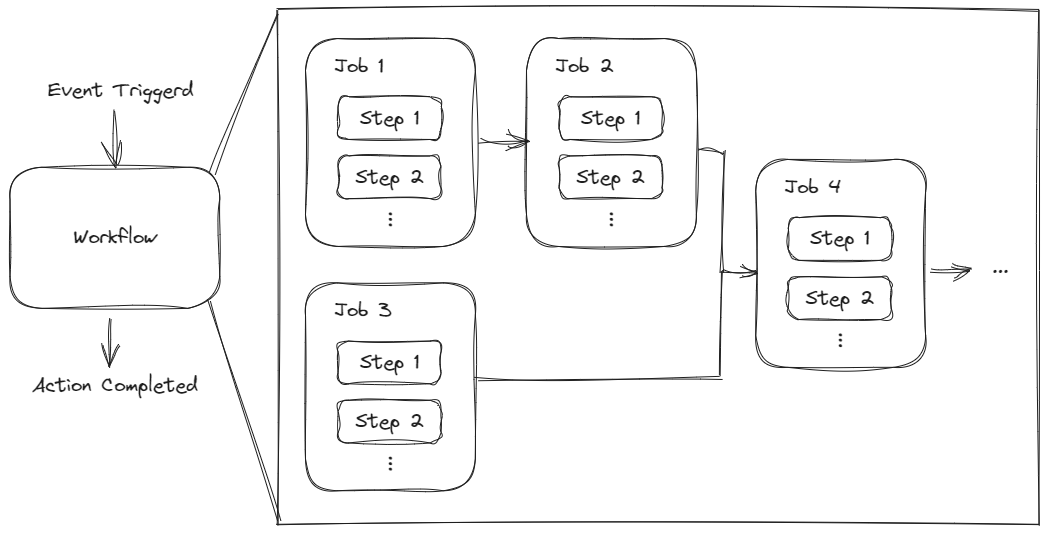
\includegraphics[width=350pt]{chapters/ap/figures/action_framework.png}
	\caption{A demonstration of GitHub Actions workflow.} \label{fig:actions_workflow}
\end{figure}

A workflow consists of jobs to be executed when a trigger happens. The jobs are executed in parallel by default (see ``job 1'' and ``job 3'' in Fig. \ref{fig:actions_workflow}), or in sequence when there are dependencies (see ``job 2'' and ``job 4'' in Fig. \ref{fig:actions_workflow}). Each job is executed in a dedicated VM or container known as a ``runner''. The running environment of a runner, such as OS, libraries, environment variables, etc., can be configured separately. In each job multiple steps can be defined. A step often corresponds with an action, such as executing a shell script. The steps in a job are executed in sequence in the configured order. Both steps and jobs can be triggered conditionally. There can be any number (at least 1) of steps in a job, any number (at least 1) of jobs in a workflow, and any number of workflows attached to a branch.

The user needs to formulate the pipelines to be executed automatically into GitHub Actions workflows.

\subsection{Supported Triggers}

It is worth mentioning that GitHub Actions can be triggered not only by repository-related events. Commonly seen triggers include
\begin{itemize}
	\item Repository-related events, such as push, pull request (most commonly seen).
	\item External events.
	\item Schedulers or timers.
	\item The user who triggers the workflow manually.
\end{itemize}

GitHub Actions provides workflow templates of different task types. There are at least the following workflow types as of this writing. They can be used for but not limited to CI/CD.
\begin{itemize}
	\item CI
	\item Deployment
	\item Testing
	\item Code quality
	\item Code review
	\item Dependency management
	\item Monitoring
	\item Automation
	\item Utilities
	\item Pages
	\item Hugo
\end{itemize}

A full list of GitHub events that can trigger GitHub Actions is given in \cite{git2025reference}.

\subsection{Jobs and Steps}

The workflows configuration files are YAML files that the user can either prepare from scratch or modify from existing templates on GitHub Marketplace, a platform where commonly used workflows are shared.

A workflow configuration file contains at least the following information:
\begin{itemize}
	\item The trigger of the workflow.
	\item The environment to execute the workflow.
	\item The actions in the workflow.
\end{itemize}

The YAML files should follow the syntax required by GitHub and be saved under \verb|.github/workflows/| so that GitHub is able to detect them as workflows and execute them accordingly.

An official demonstrative example of a GitHub workflow YAML file is given below \cite{git2025reference}. 

\begin{lstlisting}
	name: GitHub Actions Demo
	run-name: ${{ github.actor }} is testing out GitHub Actions
	on: [push]
	jobs:
	Explore-GitHub-Actions:
	runs-on: ubuntu-latest
	steps:
	- run: echo "The job was automatically triggered by a ${{ github.event_name }} event."
	- run: echo "This job is now running on a ${{ runner.os }} server hosted by GitHub!"
	- run: echo "The name of your branch is ${{ github.ref }} and your repository is ${{ github.repository }}."
	- name: Check out repository code
	uses: actions/checkout@v4
	- run: echo "The ${{ github.repository }} repository has been cloned to the runner."
	- run: echo "The workflow is now ready to test your code on the runner."
	- name: List files in the repository
	run: |
	ls ${{ github.workspace }}
	- run: echo "This job's status is ${{ job.status }}."
\end{lstlisting}

Save the above YAML file under \verb|.github/workflows/| and GitHub would recognize the workflow. Click ``Actions'' on GitHub dashboard to check the details of the workflow.

A brief introduction to YAML file syntax for GitHub Actions is given below.

In the workflow of the demonstrative example only one job, namely ``Explore-GitHub-Actions'', is defined. In practice, multiple jobs can be defined in a workflow. An example from \cite{git2025reference} is given below where 3 jobs are defined.
\begin{lstlisting}
	jobs:
	setup:
	runs-on: ubuntu-latest
	steps:
	- run: ./setup_server.sh
	build:
	needs: setup
	runs-on: ubuntu-latest
	steps:
	- run: ./build_server.sh
	test:
	needs: build
	runs-on: ubuntu-latest
	steps:
	- run: ./test_server.sh
\end{lstlisting}
Jobs are by default independent and can run in parallel unless \verb|needs| field is used just like in the above example, where ``build'' depends on ``setup'', and ``test'' on ``build''.

Commonly seen configurations in a workflow YAML file are given in Table \ref{tab:githubactions_workflow}.
\begin{table}[!htb]
	\centering \caption{Commonly seen configurations in GitHub Actions workflow.}\label{tab:githubactions_workflow}
	\begin{tabularx}{\textwidth}{lX}
		\hline
		Field & Description \\ \hline
		\texttt{name} & The static name of the workflow.  \\ 
		\texttt{run-name} & The name of an instance of run generated by the workflow.  \\ 
		\texttt{on} & The event(s) that triggers the workflow. A full list of supported events are given in \cite{git2025reference}. Multiple triggers are supported. The trigger can be configured very flexibly. \\ 
		\texttt{permissions} & Allowed r/w/x permissions for the workflow or for different triggers defined by the workflow. \\ 
		\texttt{env} & Environment variables to be used in the jobs descriptions. \\
		\texttt{defaults} & Default settings for all jobs. \\
		\texttt{concurrency} & Concurrency group of the workflow. There can be only one workflow running concurrently within a concurrency group. \\
		\texttt{jobs} & A dictionary of jobs. Each entry corresponds with a job. \\
		\hline
	\end{tabularx}
\end{table}

The \verb|jobs| field is a dictionary of jobs that run in parallel (unless \verb|needs| is used in the job description). Each entry in the dictionary corresponds with a job. The key of the entry is referred as \verb|<id>| of the job. A demonstrative example is given below.
\begin{lstlisting}
	jobs:
	job1:
	name: <something>
	runs-on: <something>
	steps:
	- <something>
	- <something>
	job2:
	name: <something>
	runs-on: <something>
	steps:
	- <something>
	- <something>
\end{lstlisting}
Commonly seen fields defined under \texttt{jobs.<id>} are summarized in Table \ref{tab:githubactions_jobs}.
\begin{table}[!htb]
	\centering \caption{Commonly seen configurations under \texttt{jobs.<id>}.}\label{tab:githubactions_jobs}
	\begin{tabularx}{\textwidth}{lX}
		\hline
		Field & Description \\ \hline
		\texttt{name} & Name of the job. \\
		\texttt{needs} & Dependencies of the job. The job executes only if its dependencies finish successfully.\\
		\texttt{if} & Prerequisite of the job. \\
		\texttt{runs-on} & The type of machine to host the job, such as \texttt{ubuntu-latest}, \texttt{windows-latest}, \texttt{macos-latest}. \\
		\texttt{environment} & Environment that the job references. \\
		\texttt{concurrency} & Concurrency group of the job. \\
		\texttt{outputs} & A map of outputs of the job to variables which can be passed to downstream jobs. \\
		\texttt{env} & A map of variables to be shared by all steps in the job. \\
		\texttt{timeout-minutes} & Maximum number of minutes of the job. \\
		\texttt{strategy} & Testing the job on multiple machines with different configurations specified by \texttt{strategy}, for example, different OSs or versions. \\
		\texttt{continue-on-error} & Preventing the workflow from failing with the job, if set to ``true''. \\
		\texttt{container} & Container configurations. If specified, some of the steps can run in the container; otherwise, all steps will run directly on the host specified by \texttt{runs-on}. Supported only if Linux OS is used. \\
		\texttt{steps} & A list of steps or actions to be executed in the job. \\
		\hline
	\end{tabularx}
\end{table}

A specific action is defined under \texttt{jobs.<id>.steps[*]}. Notice that field ``steps'' is a list, whereas each item in the list is a dictionary. Commonly seen fields of the dictionaries are summarized in Table \ref{tab:githubactions_steps}.
\begin{table}[!htb]
	\centering \caption{Commonly seen configurations under \texttt{jobs.<id>.steps[*]}.}\label{tab:githubactions_steps}
	\begin{tabularx}{\textwidth}{lX}
		\hline
		Field & Description \\ \hline
		\texttt{name} & The name of the step. \\ 
		\texttt{run} & The command to executed. \\
		\texttt{uses} & Alternative to \texttt{run}. A reusable application (known as ``action'') to be executed. \\
		\texttt{working-directory} & Working directory to run the command. \\
		\texttt{shell} & Shell to run the command. If not specified, \texttt{bash} is used on a Linux machine. \\
		\texttt{with} & A map of input variables which will be used as environment variables in the step. \\
		\texttt{env} & Environment variables of the step. \\
		\texttt{continue-on-error} & Preventing the job from failing with the step, if set to ``true''. \\
		\texttt{timeout-minutes} & Maximum number of minutes of the step. \\
		\hline
	\end{tabularx}
\end{table}

\subsection{Actions}

From earlier examples, we have seen \verb|run| used in a step to execute a command. There is a limitation to the complexity of what a command can achieve. Therefore, action is introduced. In short, action is a user-defined application that performs a complex and frequently repeated task, and it is well appreciated in GitHub Actions. The basic syntax of calling an action in a step is given below.
\begin{lstlisting}
	steps:
	- uses: <action id and version>
	with:
	<configurations>    
\end{lstlisting}
where \verb|with| is usually an optional argument that states the configuration of the action. Its contents differ from action to action.

It is worth mentioning that since actions are essentially applications, they can be packaged and shared in the community. The user can build his own actions, and he can also look for official and unofficial actions developed by other developers. For example, a collection of actions can be found at \cite{git2025actions}.

An example of an action, \verb|checkout|, is given below. It downloads the source codes in the repository to the runner. The action used in the example is provided by GitHub officials.
\begin{lstlisting}
	name:
	on:
	jobs:
	job1:
	runs-on: ubuntu-latest
	steps:
	- name: get code
	uses: actions/checkout@v4
	with:
	repository:
	ref:
	token:
	ssh-key:
	ssh-known-hosts:
	ssh-strict:
	ssh-user:
	persist-credentials:
	path:
	clean:
	filter:
	sparse-checkout:
	sparse-checkout-cone-mode:
	fetch-depth:
	fetch-tags:
	show-progress:
	lfs:
	submodules:
	set-safe-directory:
	github-server-url:
\end{lstlisting}
where \verb|uses| is used to indicate an action, and \verb|actions/checkout@v4| is the identifier and version of the action. The \verb|with| field (optional) is then used to configure the action if needed. The content of the configuration depends on the specific action in use. The details of the configurations about \verb|checkout@v4| can be found at \cite{git2025actions} and are not covered in this notebook. 

There are many tasks that can be done via actions. To just name a few,
\begin{itemize}
	\item Retrieve code, such as \verb|checkout|.
	\item Upload or download artifact, such as \verb|upload-artifact|, \verb|dowload-artifact|.
	\item Install software, such as \verb|setup-node|, \verb|setup-python|, \verb|setup-dotnet|.
\end{itemize}
There are many more wonderful actions on the market, many of which can be used free-of-charge.

\subsection{Contexts}

The following syntax 
\begin{lstlisting}
	${{ <context>.<information> }}
\end{lstlisting}
can be used to access GitHub Actions contexts in the workflow configuration files. Examples have been given in earlier sections. \mync{GitHub Actions contexts} are collections of read-only information available to the workflow configuration. There are many contexts defined and they cover a large range of topics regarding the workflow, the job, the runner, the step, environment variables, secrets, and many more.

As a recap, in the earlier example the following information is retrieved.
\begin{itemize}
	\item \verb|${{ github.event_name }}|: the trigger of the event.
	\item \verb|${{ runner.os }}|: the OS of the runner.
	\item \verb|${{ github.ref }}|: branch name.
	\item \verb|${{ github.repository }}|: repository name.
\end{itemize}

The information from contexts can be used in if-else statements to direct the workflow. Another common practice is to use an expression, such as
\begin{lstlisting}
	${{ toJSON(github) }}
\end{lstlisting}
to convert contexts into JSON strings, cache them in environment variables, and use them in the commands.

\subsection{Costs}

Last but not least, GitHub Actions may generates additional costs. This is because the workflows are executed on runners based on GitHub's servers, consuming its CPU, memory and storage. As of this writing, additional cost is generated only if all of the below are true:
\begin{itemize}
	\item Private repository.
	\item The workflows are executed on GitHub servers. Notice that it is possible to execute workflows using on-premises servers, in which case GitHub Actions becomes a free service.
	\item CPU, memory and storage usages go beyond the free-tier threshold.
\end{itemize}

If all the above criteria are met, the user pays GitHub for the storage and computational consumption. He can select either prepaid mode (fixed bill, limited consumption per month) or postpaid mode (unfixed bill, unlimited consumption per month).

The running environment also affects the cost. It is often more expensive if the workflow needs to run on Windows or MacOS than if it can run on Linux due to the licensing fee. As of this writing, Windows and MacOS introduce a computational cost multiplier of $2$ and $10$ respectively comparing with Linux.
